\documentclass[12pt]{article}
 
\usepackage[utf8]{inputenc}
\usepackage[brazilian]{babel}
\usepackage{fontenc}
\usepackage{graphicx} 
\usepackage{listings}
\usepackage{xcolor}
\usepackage{indentfirst}
\usepackage{pdflscape}
\usepackage[bottom=3cm,top=3cm,left=3cm,right=3cm]{geometry} 
\usepackage[pdftex]{hyperref} %permitir \url

\usepackage{wallpaper}
\usepackage{subfig}

\usepackage{fancyhdr}
\pagestyle{fancy}
\fancyhf{}
\rhead{QXCode}
\lhead{Playfair}
\fancyfoot[R]{\thepage}
%\rfoot{Page \thepage}


\usepackage[absolute]{textpos}


\lstset{
    language=java,
%    language=c++,
    keywordstyle=\bfseries\ttfamily\color[rgb]{0,0,1},
    identifierstyle=\ttfamily,
    commentstyle=\color[rgb]{0.133,0.545,0.133},
    stringstyle=\ttfamily\color[rgb]{0.627,0.126,0.941},
    showstringspaces=false,
    basicstyle=\small,
    tabsize=2,
    breaklines=true,
    frame=single
}



\renewcommand{\tt}[1]{\lstinline|#1|}
\renewcommand{\bf}[1]{\textbf{#1}}


\begin{document}

\ThisULCornerWallPaper{1}{./imagens/header}

\begin{textblock}{15}(0.4, 0.4)
\noindent
\begin{center}
\LARGE{\bf{QXCode - Quixadá Coding Team}}\\
\large{\bf{Fundamentos de Programação}} \\
\large{\bf{\today}}
\end{center}
\end{textblock}

\title{\bf{Playfair \\ Cifragem de Blocos}}

\author{
David Sena \thanks{sena.ufc@gmail.com}
}

\date{}

\maketitle
\thispagestyle{empty}

%#################################################################
%#################################################################
%#################################################################
%#################################################################


\section{Instruções Gerais}
O objetivo desse trabalho é a construção de um programa que realize a cifragem e a decifragem de um texto utilizando a criptografia de Playfair. Ele demandará de conhecimento dos assuntos de strings, matrizes e um pouco de arquivos. 

\begin{figure}[hf]
\centering
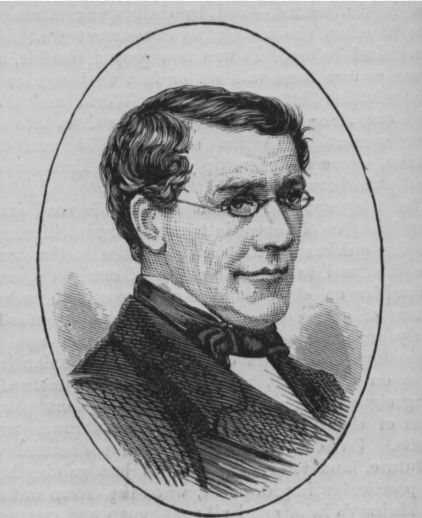
\includegraphics[width=0.3\linewidth]{./imagens/author}
\caption*{Autoria de Charles Wheatstone}
%\label{fig:playfair}
\end{figure}


\section{A cifra de Playfair}

O conteúdo dessa seção é retirada do site abaixo. Apenas os conteúdos mais importantes foram copiados pra cá. Sugiro que você leia na íntegra no site:
\url{http://www.numaboa.com.br/criptografia/substituicoes/poligramicas/1041-playfair}

\subsection{História}

Apesar do nome do Barão de Playfair estar associado a uma das cifra clássicas mais conhecidas, foi seu amigo, o cientista Charles Wheatstone, quem a concebeu. Após sua criação em 1854, o barão conseguiu que o governo britânico adotasse oficialmente o uso da cifra - daí o nome Cifra "de" Playfair.

A Playfair é uma cifra de bloco primitiva, usando alguns princípios comuns às cifras de bloco atuais. O melhor meio de se aproximar da criptologia moderna, sem ter que enfrentar a teoria dos números e a matemática, é entendendo a Playfair.

As letras são tomadas duas a duas, e aplicadas a uma grade de 5 por 5 que contém o alfabeto cifrante.

A Playfair possui outras vantagens: não precisa de tabelas ou dispositivos complicados, possui uma palavra-chave que pode ser memorizada ou trocada com facilidade, é muito fácil de ser implementada e pouco sujeita a erros. Devido a estas características o sistema é perfeito para ser usado como uma "cifra de campo".

\subsection{Preparando o texto}


A preparação do texto claro é extremamente fácil: basta formar grupos de 2 letras, os blocos digrâmicos. Cada bloco receberá um tratamento de acordo com as regras cifrantes (veja abaixo). O texto claro que será cifrado com a Playfair é:

MORRO MAS SAPRENDO C 

Preparamos o texto para ser cifrado:
MO RR OM AS SA PR EN DO  OC

De imediato notamos que o último bloco ficou com apenas uma letra e que existe um bloco com letra dupla (RR). Letras repetidas impedem que a cifra possa ser aplicada corretamente. Nestes casos, convenciona-se uma letra de separação. Geralmente são usados preferencialmente o X e o Z, caso sejam dois XX. Caso falte uma letra no final, adiciona-se X ou Z. Corrigindo os blocos obtemos:
\begin{verbatim}
MO RX RO MA SX SA PR EN DO CX
\end{verbatim}

\subsection{A matriz de cifragem}

O alfabeto cifrante proposto por Wheatstone fica disposto numa grade de 5 por 5. Como o alfabeto latino possui 26 letras, é preciso eliminar uma das letras. Eliminaremos o W. 

Além disto, para facilitar a memorização do cifrante, Wheatstone sugeriu começar o preenchimento da grade com uma palavra-chave. O restante das células é preenchido com as letras faltantes em ordem alfabética.

No nosso exemplo usaremos a palavra-chave "POWER RANGER". Ignoraremos o W e retiraremos os duplicados. Ficamos com "POERANG". Preenchemos a
grade começando de cima pela esquerda. Depois
colocamos o resto do alfabeto em ordem alfabetica.

Resultado:
\begin{verbatim}
P O E R A
N G B C D
F H I J K
L M Q S T 
U V X Y Z
\end{verbatim}

\section{Cifragem}
As letras de um bloco podem ter apenas 3 localizações na grade: estão na mesma linha, estão na mesma coluna ou estão em linhas e colunas diferentes. Portanto, existem apenas 3 regras que devem ser aplicadas aos blocos digrâmicos:

1. Letras na mesma linha são substituídas pelas letras à sua direita. Caso uma das letras do bigrama esteja na última coluna da grade, "roda-se a linha" e utiliza-se a letra da primeira coluna.
\begin{verbatim}
    Ex: PR > OA, CG > DB, ZV > UX, ZY > UZ
\end{verbatim}
2. Letras na mesma coluna são substituídas pelas letras abaixo delas. Caso a letra esteja na última linha, "roda-se a coluna" e utiliza-se a letra da primeira linha.
\begin{verbatim}
    Ex: PF > NL, PU > NP, VM > OV, FN > LF
\end{verbatim}
3. Letras em linhas e colunas diferentes: as letras do bigrama formam um "quadrilátero" e são substituídas pelas letras posicionadas nos cantos contrários do quadrilátero.
\begin{verbatim}
    Ex: PG > ON, GP > NO, PB > EN, ZP > UA
\end{verbatim}
\subsection{Aplicando a grade}

Nosso texto e nossa grade ficarm assim.

\begin{verbatim}
Texto claro:
MO RX RO MA SX SA PR EN DO CX

Grade:

P O E R A
N G B C D
F H I J K
L M Q S T 
U V X Y Z
\end{verbatim}

Cifrando usando as regras temos:


\begin{verbatim}
Texto claro:
MO RX RO MA SX SA PR EN DO CX
Texto cifrado:
VG EY AE TO QY TR OA PB GA BY
\end{verbatim}

Para descriptografar é só fazer as operações contrárias.

\section{O programa}

Você deve fazer criptografar e descriptografar. Ao ser executado ele receberá o nome do arquivo
que contém o texto por parametro e perguntará a senha ao usuário. Ele mostrará o texto processado
na tela.


\begin{verbatim}
--Conteúdo de texto.txt
MORRO MAS SAPRENDO C 

--Rodando o programa:
# ./cifrar texto.txt
>> Digite a chave:
<< POWERRANGER
>> O texto cifrado eh:
VG EY AE TO QY TR OA PB GA BY



--Conteudo do arquivo cifra.txt
VG EY AE TO QY TR OA PB GA BY

--Rodando o programa de decifrar
# ./decifrar cifra.txt
>> Digite a chave:
<< POWERRANGER
>> O texto cifrado eh:
MO RX RO MA SX SA PR EN DO C

\end{verbatim}

\end{document}

